\chapter*{Introduction}
\addcontentsline{toc}{chapter}{1. Introduction} % Manual index entry
% Hablar de la empresa
% Hablar del objetivo del trabajo
% Comentar la estructura del documento

In today's world, where efficiency and strategic decision-making make the difference 
between moving forward or falling behind, task management within a company plays a fundamental role.
Many times, behind a good product or service, there is precise planning, careful coordination, and optimal use of the available resources.
In this context, mathematics, and more specifically, optimization, becomes a powerful tool for transforming complexity into clear and applicable solutions.

This work arises with the intention of building a bridge between theoretical knowledge and its practical application in the business environment.
We have chosen Intercrop, a company based in Cartagena specializing in the agri-food sector, as our case study.
Intercrop stands out for its commitment to sustainability and innovation in agricultural production, but like any company, it faces logistical and organizational challenges that require smart solutions.
Intercrop not only operates at a national level but also maintains a close relationship with the international market.
It exports a significant part of its production to various European countries, which demands high quality standards, strict deadline compliance, and a well-structured logistics system.
This international dimension adds complexity to its operational management, as it must coordinate agricultural tasks with transport schedules, phytosanitary requirements, and commercial commitments abroad.
All of this makes the company a particularly interesting environment for applying optimization tools that can help improve planning and efficiency in a real and demanding context.

Through this project, we will address the task scheduling problem within the company. The goal is to design an optimization model that efficiently organizes activities, taking into account real-world constraints: time, limited resources, task dependencies, and other logistical factors.
This process will not only allow us to provide the company with a proposal for improvement, but also to apply in a practical way the mathematical concepts learned in the classroom, especially those related to linear programming and optimization.


\vspace{10mm}
\begin{figure}[ht!]
    \centering
    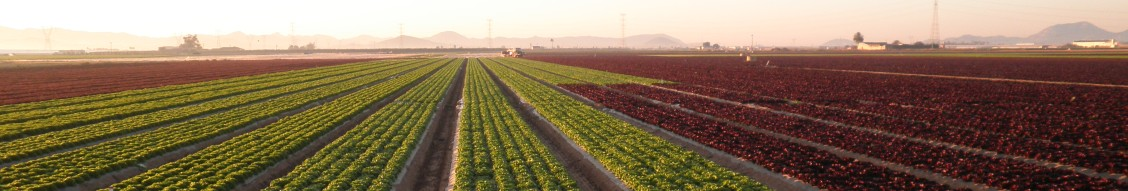
\includegraphics[width=1\textwidth]{img/campitos_lindos.jpeg}
    %\caption{Intercrop, empresa de referencia para el estudio de planificación de tareas agrícolas.}
    \label{fig:campitos_lindos}
\end{figure}

\chapter*{Problem Statement}
\addcontentsline{toc}{chapter}{2. Problem Statement} % Manual index entry
% Explicación en "leguaje natural" del problema
% Simplificaciones
% Descripción de las tareas

Task planning in the agricultural sector represents a significant logistical and operational challenge,  
especially for companies operating under a made-to-order production model, as is the case with Intercrop.  
This company, located in Cartagena and specialized in horticultural products, organizes its production based on seasonal demand.  
During the summer campaign, both the quantity of product to be supplied and the specific delivery dates are established in advance.  
This means that all planning—from cultivation and growth to \gls{harvest}$^{(*)}$ and distribution—must be precisely aligned to meet deadlines,  
ensure the quality of the fresh product (with a shelf life of seven to ten days), and minimize operational costs.

Given the data of an order, we must take into account the number of \gls{raised bed}s$^{(*)}$ that need to be \gls{transplanted}$^{(*)}$ for each variety in order to fulfill it.  
A small surplus is transplanted as a precautionary measure to ensure the required amount is met.  
This surplus does not need to be considered in the planning, as it generates no additional cost and is later offered to the clients.
 

The objective of this work is to address, from a mathematical and practical perspective, the problem of agricultural task scheduling within the real-world context of this company.  
To this end, we will focus on two main crops: lettuce and spinach, including two varieties of lettuce and five varieties of spinach.

\begin{itemize}
    \item \textbf{Lettuce}: it is grown in two varieties, one with curly leaves (Apollo, Fig. \ref{fig:apollo}) and the other with smooth leaves (Knox Cos, Fig. \ref{fig:knox}). The curly leaf lettuce is more delicate and requires special care. In contrast, the smooth leaf lettuce is more resilient and better suited to less precise conditions.
	\item \textbf{Spinach}: five varieties are grown: one with small leaves, both in its common version (Baby Spinach, Fig. \ref{fig:baby}) and in its organic version; medium-sized leaves in both green (Teen Spinach, Fig. \ref{fig:teen}) and a more reddish color (Red Spinach, Fig. \ref{fig:red}). There is also a flat-leaf variety intended for soup preparation (Soup Spinach, Fig. \ref{fig:soup}).
    Regarding differences in treatment, there are no substantial changes in care.
\end{itemize}
The main difference between the varieties we are considering is the cultivation time required for each of them.
\begin{figure}[ht!]
    \centering

    \begin{minipage}[b]{0.45\textwidth}
        \centering
        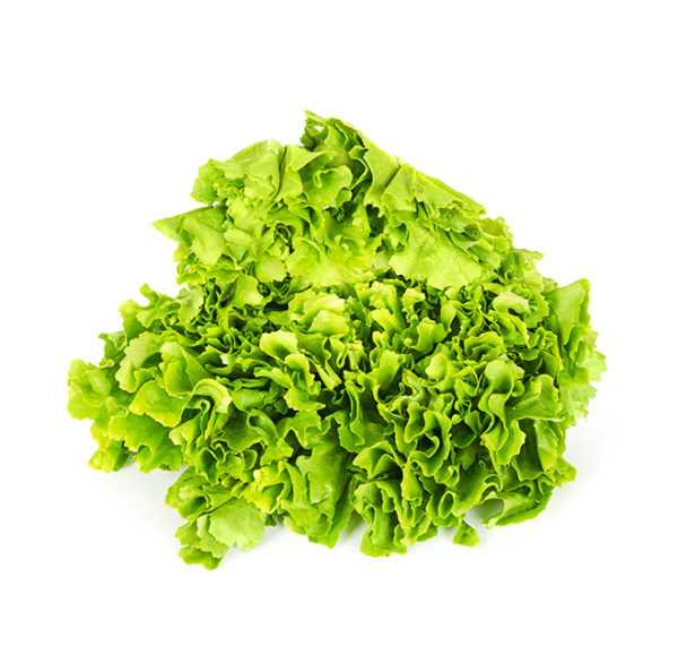
\includegraphics[width=0.7\textwidth]{img/lechuga_apollo.png}
        \caption{Lettuce variety Apollo.}
        \label{fig:apollo}
    \end{minipage}
    \hfill
    \begin{minipage}[b]{0.45\textwidth}
        \centering
        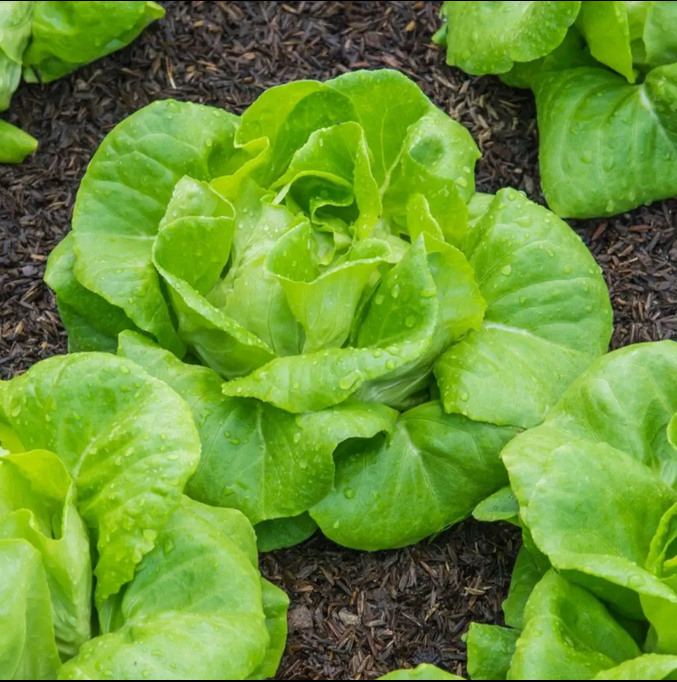
\includegraphics[width=0.6\textwidth]{img/lechuga_knox.png}
        \caption{Lettuce variety Knox Cos.}
        \label{fig:knox}
    \end{minipage}

\end{figure}

\begin{figure}[ht!]
    \centering

    \begin{minipage}[b]{0.45\textwidth}
        \centering
        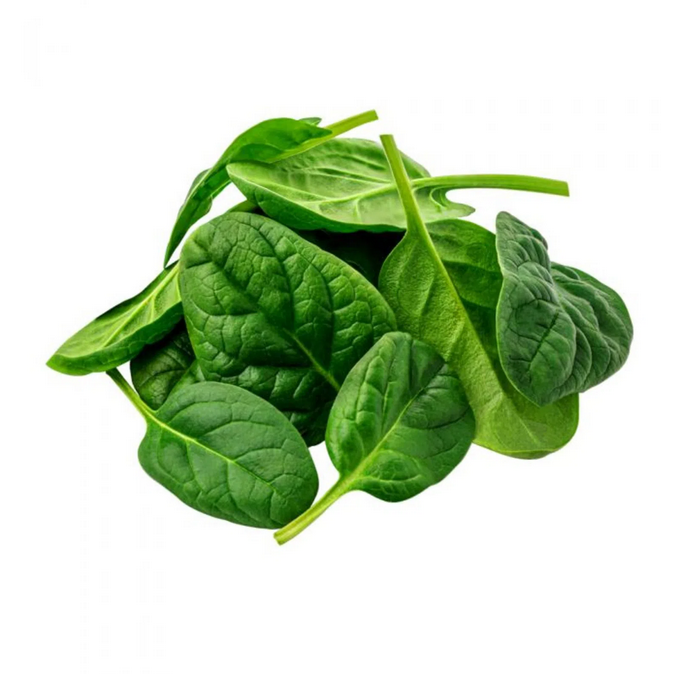
\includegraphics[width=0.6\textwidth]{img/baby_spinach.png}
        \caption{Variety Baby Spinach.}
        \label{fig:baby}
    \end{minipage}
    \hfill
    \begin{minipage}[b]{0.45\textwidth}
        \centering
        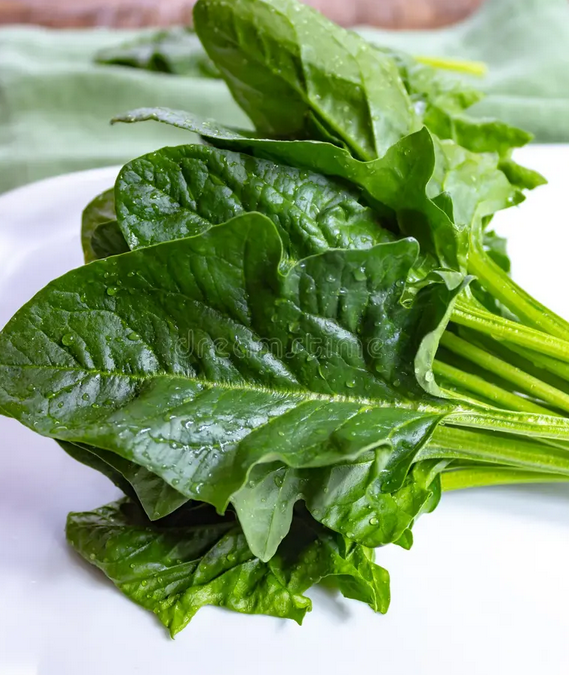
\includegraphics[width=0.5\textwidth]{img/teen_spinach.png}
        \caption{Variety Teen Spinach.}
        \label{fig:teen}
    \end{minipage}
    \begin{minipage}[b]{0.45\textwidth}
        \centering
        
\includegraphics[width=0.6\textwidth]{img/red_spinach.jpg}
        \caption{Variety Red Chard.}
        \label{fig:red}
    \end{minipage}
    \begin{minipage}[b]{0.45\textwidth}
        \centering
        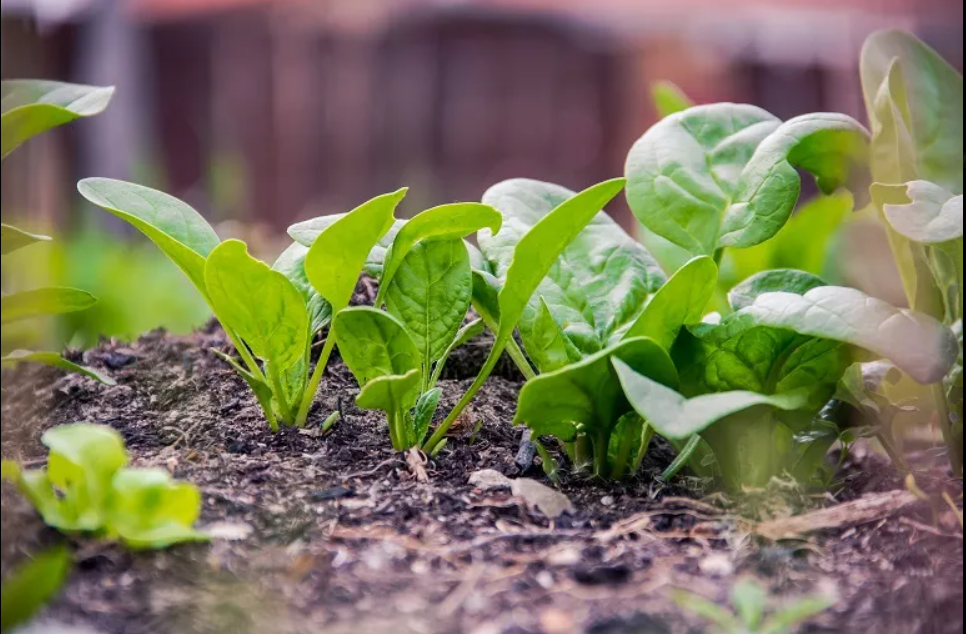
\includegraphics[width=0.6\textwidth]{img/soup_spinach.png}
        \caption{Variety Soup Spinach.}
        \label{fig:soup}
    \end{minipage}
\end{figure}

\newpage
Before breaking down the tasks involved in the cultivation process, it is important to highlight a fundamental difference between the two products.
Lettuce is grown through transplanting: seeds are sent to a nursery and later the seedlings are transplanted into the field.
In the case of spinach, the direct sowing method is used, placing the seeds directly into the soil.
Due to the different nature of these methods, each crop will have its own specific timelines and requirements, which will influence task scheduling.

The list of tasks required to complete a cultivation cycle is as follows:
\begin{enumerate}
    \item Soil preparation: a set of initial tasks in which the soil is broken up and turned to aerate it, and fertilized to ensure it is properly conditioned before cultivation.  
Next, using specialized machinery, the cultivation surfaces are arranged into \gls{raised bed}s$^{(*)}$.

\item Install paper: sheets are installed to prevent the growth of weeds, thereby reducing competition with the main crop.

\item \gls{Sowing}$^{(*)}$ or transplanting: depending on the crop variety, seeds are sown directly or previously grown seedlings from an external company are transplanted.

\item Irrigation: installation of sprinkler irrigation systems on the \gls{slope}s$^{(*)}$ of the raised beds, essential for maintaining the crop.

\item Placing \gls{hoops}$^{(*)}$: metal arches are installed over the crops to support the subsequent protective covering.

\item Installing \gls{mesh}$^{(*)}$: the hoops are covered with a polyamide mesh that protects the crops and helps maintain the proper temperature for their development.

\item Removing mesh: once the crop has matured, the protective mesh is removed.

\item Removing hoops: after the mesh has been taken off, the metal hoops are dismantled.

\item Removing irrigation: the previously installed irrigation system is disassembled.

\item Harvesting: final stage of the process, which can be done manually (with workers placing the products into boxes) or through automated methods.

\end{enumerate}

Each of these tasks is carried out using different machinery, generally implements pulled by tractors, which implies different working speeds depending on the equipment used.  
In addition, Intercrop organizes its production through specialized work groups, which are not hired at the beginning of the season but are gradually incorporated as their tasks become necessary.  
This structure allows the company to adapt to the needs of the process, but it also creates delays when one group has to wait for another to finish before continuing.

During our visit to the company, we observed that this lack of synchronization between groups often leads to idle time: periods in which workers are present but unable to act,  
as the previous task has not yet been completed. These hours, though unproductive, are counted in the total working hours and represent a direct economic cost to the company.

The main objective of this proposal is to develop a scheduling model that minimizes unproductive time between work groups,  
while ensuring that the committed delivery deadlines are met. More efficient coordination of tasks would lead to significantly better resource utilization,  
reducing waiting times and increasing overall system productivity.


\section*{Model Simplifications}
\addcontentsline{toc}{section}{2.1. Model simplifications} % Manual index entry

In order to approach the problem from a mathematical and computational perspective, 
it has been necessary to make certain simplifications, which allow us to focus on the essential aspects of the process without loss of generality:
\begin{itemize}
    \item Scale reduction: the model is applied to only two farms, one dedicated to lettuce and the other to spinach.  
	This decision allows us to work with two distinct and representative production lines, without the need to model the company's entire global operation.
	
	\item Medium-sized farms: it is assumed that both farms have similar and average dimensions, which allows the same planning scheme to be applied  
	to each one without specific considerations regarding size or shape.
	\item Homogeneous cultivation: it is assumed that, within each farm, the tasks required for the care of the most delicate variety will be carried out.  
	Therefore, we will assume that in the farm dedicated to lettuce, all tasks from the previously mentioned list are performed, while in the case of spinach, the use of mesh and hoops will be omitted.  
	Thus, the first farm will carry out all 10 tasks listed earlier, while the spinach farm will only perform tasks 1, 3, 4, 9, and 10.
	
	\item Independent work groups: each crop is managed by a different work group, with its own machinery and resources.  
	This allows both production lines to be treated in a parallel and simplified manner.
	
	\item Unit conversion: the machinery speeds, originally provided by the company in kilometers per hour, have been converted to beds per hour  
	to simplify the formulation and adapt the units to the structure of the model.
	
	\item Ideal conditions: the model is developed under a scenario with no mechanical failures or weather-related interruptions.  
	In other words, it is assumed that all tasks are completed within the estimated time and that there are no delays due to external factors.
	
	\item Fixed workday: a standard workday of 8 hours is considered, with no seasonal changes or holidays.
\end{itemize}
 
These simplifications do not eliminate the complexity of the problem, but they allow us to structure a realistic, functional, and computationally viable model that can serve as a foundation for future expansion or practical implementation.


\chapter*{Data}
\addcontentsline{toc}{chapter}{4. Data} % Manual index entry
% Explicación de los datos
% Tablas
During our visit to the company, we were able to observe their working methods. This helped us gain a clear understanding of the workflow we needed to design  
and identify the data we would require. Subsequently, the company provided us with the specific data we requested.

For our study, we assume that the farms have a rectangular shape. We consider the lettuce farm to measure 100 x 300 meters,  
while the spinach farm measures 180 x 300 meters. Each raised bed is 1.6 meters wide, with lateral furrows of 0.4 meters to allow machinery to pass.  
This means each path has dimensions of 2 x 300 meters.  
As a result, the first farm contains 50 paths with their respective 50 raised beds, while the second contains 90 paths with 90 raised beds.

The tasks are mechanized, as each is carried out by a tractor equipped with a different implement.  
Therefore, we need to know the speed the tractor can reach depending on the implement used for each task.  
Although the company provided these speeds in kilometers per hour (km/h), we converted them to beds per hour to simplify our model formulation.

 \begin{table}[ht!]
    \centering
    \begin{minipage}{0.48\textwidth}
        \centering
        \begin{tabular}{|c|c|c|}
            \hline
            \rowcolor{gray!30} \textbf{\textcolor{grey3}{TASK}} & \textbf{\textcolor{grey3}{SPEED}} &  \textbf{\textcolor{grey3}{WORKERS}}\\ 
            \hline
            Soil preparation   & 2 & 4 \\ \hline
            Install paper      & 4 & 2\\ \hline
            Transplant         & 3 & 6\\ \hline
            Sow                & 4 & 5\\ \hline
            Install irrigation & 3 & 2 \\ \hline
            Install hoops      & 3 & 3 \\ \hline
            Install mesh       & 3 & 2 \\ \hline
            Remove mesh        & 4 & 2 \\ \hline
            Remove hoops       & 3 & 2 \\ \hline
            Remove irrigation  & 3 & 2 \\ \hline
            Harvest seeds      & 3 & 7 \\ \hline
            Harvest plants     & 2 & 14 \\ 
            \hline
        \end{tabular}
        \caption{Tasks, speeds, and number of workers per task.}
        \label{tab:tareas}
    \end{minipage}
    \hfill
\end{table}
Our scheduling is designed to organize one month of work. Considering a standard workday of 8 hours,  
we work with a total of 240 hours per month.

On the other hand, workers join the campaign in a staggered manner. Each of them is specialized in a specific task,  
leading to the formation of specialized work groups.  
The number of workers per group varies depending on the task assigned.

Another important aspect to consider is the time required for each variety to grow. The company provided this information in days,  
although they noted that in the case of spinach varieties, the growth time is not fixed, as it depends largely on the amount of solar radiation received.  
For this reason, they gave us a range of days during which each variety is typically harvested, indicating which ones show greater or lesser variability in growth.  
Using this data, we estimated the optimal time for harvesting.  

Moreover, since we work in hours, we converted the time scale: each day indicated by the company is expressed in our formulation as an eight-hour period.  
This way, we adjusted the growth times to fit our scheduling framework.

\begin{table}[ht!]
    \centering
    \begin{minipage}{0.48\textwidth}
        \centering
        \begin{tabular}{|c|c|c|}
            \hline
            \rowcolor{gray!30} \textbf{\textcolor{grey3}{RANGES}} & \textbf{\textcolor{grey3}{DAYS}} &  \textbf{\textcolor{grey3}{HOURS}}\\\hline 
            \hline
            Baby spinach   & 24 & 192 \\ \hline
            Baby spinach organics  & 26 & 208\\ \hline
            Red Spinach              & 22 & 176\\ \hline
            Teen Spinach           & 23.4 & 187\\ \hline
            Soup Spinach & 25.4 & 203 \\ \hline
            Knox Cos     & 22 & 176 \\ \hline
            Apollo      & 24 & 192 \\ 
             
            \hline
        \end{tabular}
        \caption{Table of Varieties and Growth Time}
        \label{tab:Variedades-crecimiento}
    \end{minipage}
    \hfill
\end{table}

The company provided us with the general annual order they need to fulfill. Since the campaign lasts ten months, we divided the order  
to obtain the equivalent for the time period we are working with. Additionally, the company informed us of the number of seeds  
required to meet the order, as well as the yield obtained when planting them.  
With this information, we were able to estimate the number of kilograms planted in each raised bed.
\begin{table}[ht!]
    \centering
    \begin{minipage}{0.48\textwidth}
        \centering
        \begin{tabular}{|c|c|c|}
            \hline
            \rowcolor{gray!30} \textbf{\textcolor{grey3}{RANGES}} & \textbf{\textcolor{grey3}{kilos pedidos}} & \textbf{\textcolor{grey3}{kg/meseta}}\\\hline 
            \hline
            Baby spinach   & 228235 & 5087\\ \hline
            Baby spinach organics  & 22574 & 5543\\ \hline
            Red Spinach              & 27560 & 2197\\ \hline
            Teen Spinach           & 25474 & 2450\\ \hline
            Soup Spinach & 30896 & 2059\\ \hline
            Knox Cos     & 43459 & 6421\\ \hline
            Apollo      & 15928 & 3243 \\          
            \hline
        \end{tabular}
        \caption{Table of Varieties and Order in Kilograms}
        \label{tab:Variedades-kilos}
    \end{minipage}
    \hfill
\end{table}

Since our formulation is based on raised beds, we only need to determine how many raised beds must be transplanted for each variety  
in order to fulfill the order on time and in the required quantity.

 \begin{table}[ht!]
    \centering
    \begin{minipage}{0.48\textwidth}
        \centering
        \begin{tabular}{|c|c|}
            \hline
            \rowcolor{gray!30} \textbf{\textcolor{grey3}{RANGES}} & \textbf{\textcolor{grey3}{mesetas}}\\\hline
            \hline
            Baby spinach   & 45 \\ \hline
            Baby spinach organics   & 5\\ \hline
            Red Spinach             & 13\\ \hline
            Teen Spinach            & 11\\ \hline
            Soup Spinach & 16 \\ \hline
            Knox Cos     & 36 \\ \hline
            Apollo      & 14 \\             
            \hline
        \end{tabular}
        \caption{Table of varieties and raised beds}
        \label{tab:Variedades}
    \end{minipage}
    \hfill
\end{table}
For the sake of simplicity, we assume that the raised beds assigned to each variety are consecutive.  
For example, those for *Baby Spinach* range from bed 1 to 50, those for *Baby Spinach Organics* from bed 46 to 50, and so on.


\chapter*{Formulation}
\addcontentsline{toc}{chapter}{3. Formulation} % Manual index entry
% Variables
% Funcion objetivo
% Restricciones

To address agricultural task scheduling in a structured and optimizable manner, we have developed a mathematical model that formally describes the constraints, resources, and objectives of the problem at hand.  
This formulation will enable us to find an efficient task allocation that minimizes unproductive time, ensuring that all tasks are performed in accordance with their technical and temporal requirements.

\section*{Parameters}
\addcontentsline{toc}{section}{3.1. Parameters} % Manual index entry
The first step is to define a set of parameters that accurately represent the working environment in both fields, each dedicated to a different product (lettuce and spinach),  
and therefore, as previously mentioned, with distinct task sequences.


\subsubsection{Set of Tasks}
\begin{itemize}
    \item Set of tasks for Field 1, dedicated to lettuce:

        $T_1$:= \{preptierra1,papel1,plantar1,ponerriego1,ponermalla1,quitarmalla1,quitarriego1,cosecha1\}    
    \item Set of tasks for Field 2, dedicated to spinach:

        $T_2$:= \{preptierra2,sembrar2,ponerriego2,quitarriego2,cosechar2\}
\end{itemize}

\subsubsection{Varieties and Growth Times}

Each field contains different varieties of the same product, which are distributed homogeneously across the raised beds:


\[\begin{aligned}
        Q_1&:={apollo, knoxcos}\\
        Q_2&:={babyspinach, teenspinach, babyspinachorganic, soupspinach, redspinach}
    \end{aligned}\]

Each of them will have a specific growth time:
\[\begin{aligned}
        S_1&:=\{s_{apollo},s_{knoxcos}\}\\
        S_2&:=\{s_{babyspinach}, s_{teenspinach}, s_{babyspinachorganic}, s_{soupspinach}, s_{redspinach}\}
    \end{aligned}\]



\subsubsection{Raised beds and Time Horizon}

For each field, we define the corresponding set of raised beds ($M_j$), the total number of raised beds ($N_j$),  
and the set of working hours ($H$) available during the order period:
    \[\begin{aligned}
        M_1&:=\{1....50\}\\
        M_2&:=\{1....90\}\\
        N_1&:=50\\
        N_2&:=90\\
        H&:=\{1...240\}
    \end{aligned}\]

\subsubsection{Task Time Availability}

Tasks are not active throughout the entire time horizon; they are introduced gradually.  
Moreover, since each field has a different set of available tasks, we define a schedule family for each one:

\[\begin{aligned}
    H_1 &:= \{H_{preptierra1},H_{papel1},H_{plantar1},H_{ponerriego1},H_{ponermalla1},H_{quitarmalla1},H_{quitarriego1},H_{cosecha1}\}\\
    H_2 &:= \{H_{preptierra2},H_{sembrar2},H_{ponerriego2},H_{quitarriego2},H_{cosechar2}\}   
\end{aligned}\]    

\subsubsection{Working Speed of Machines}

Each task is performed using different machinery, and therefore at different speeds. These are expressed in beds per hour:
\begin{center}
$V_{i_1} :=$ maximum number of beds per path in one hour, $\forall i_1 \in T_1$

$V_{i_2} :=$ maximum number of beds per path in one hour, $\forall i_2 \in T_2$
\end{center}




\subsubsection{Personnel Assigned to Each Task}

Each task has an assigned work group, which includes the number of people required for its execution.
\begin{center}
    $P_{i_1}$ := number of people assigned to task $i_1 \in T_1$

    $P_{i_2}$ := number of people assigned to task $i_2 \in T_2$    
\end{center}


\section*{Decision Variables}
\addcontentsline{toc}{section}{3.2. Decision Variables} % Manual index entry
To correctly model the execution of tasks on each raised beds and at each moment within the time horizon, the following binary variable is defined:
\[
\begin{aligned}
    x_{i_j,k,l} = 
    \begin{cases} 
        1 & \text{if task } i \text{ is performed on raised bed } k \text{ at hour } l \\
        0 & \text{otherwise}
    \end{cases}
\end{aligned}
\]

where:
\begin{itemize}
    \item $i_j$ represents a task belonging to the set $T_j$.
    \item $k \in M_j$ represents one of the beds in field $j$.
    \item $l \in H_{i_j}$ represents an hour within the availability interval of task $i_j \in T_j$.
\end{itemize}


On the other hand, to capture waiting times or idle hours between tasks  
(i.e., when a work group is available but cannot start because a previous task has not yet been completed on that raised bed), we define the following variable:

\[
\begin{aligned}
    w_{i_j l} = 
    \begin{cases} 
        1 & \text{if task } i_j \in T_j \text{ can still be assigned to a raised bed at hour } l \in H_{i_j} \\
        0 & \text{otherwise}
    \end{cases}
\end{aligned}
\]


\section*{Constraints}
\addcontentsline{toc}{section}{3.3. Constraints} % Manual index entry
The agricultural scheduling model must ensure that task execution aligns with operational capacities,  
the available calendar, and the logical order of the production process.  
To achieve this, the following constraints have been defined:
\begin{itemize}
    \item We cannot assign more beds per hour than what the task allows.  
    The execution speed of each task is determined by the tractor; therefore, we cannot assign more raised beds than can be handled in one hour.  
    To enforce this, we fix a specific hour and task and iterate over all raised beds.  
    The total number of assignments must not exceed the maximum number of raised beds the machinery can process per hour.
    \[
            \sum_{k\in M_j}x_{i_j kl} \leq V_{i_j} \quad \forall i_j \in T_j, \ l\in H_{i_j}
        \]
    \item Each task can only be performed once on the raised beds where it is applicable.  
        To ensure this, we fix a raised bed and a task, and require that the sum over all hours in its schedule equals 1.  
        Otherwise, the task would either not be performed (if the sum is 0) or performed more than once (if the sum exceeds 1).
        
        \[
	        \sum_{l\in H_{i_j}}x_{i_j kl} =1 \quad \forall i_j \in T_j , k \in M_j
        \]
    \item Tasks follow a specific order that must be respected.  
        We cannot perform the next task on a raised bed without having completed the previous one.  
        We must ensure that the preceding task has been completed on that raised bed before the current one can begin.
        
        To enforce this, we fix a raised bed, a task, and a time, and verify that the previous task has been executed during the preceding hours.
         
        \[
	        x_{i_j kl} \leq \sum_{l' \in H_{prev(i_j)}, l'<l}x_{prev(i_j)kl'} \quad \forall i_j\in T_j/\{first(T_j)\}, k\in M_j, l \in H_{i_j}
        \]
	
    \item The growth period of each variety must be respected. 
        Once irrigation is in place, the plant begins to grow,  
        and it must remain undisturbed for a certain period until it reaches maturity. This duration depends on the specific variety.  
        Only after this growth time has elapsed can the subsequent tasks be performed.
        
        \[
	        x_{\text{quitarmalla}1 kl} \leq \sum_{l'\in H_{\text{ponerriego}1}, l'<l-s_{apollo}}x_{\text{ponerriego}1kl'} \quad k\in \{1, ..., 36\}, l\in H_{\text{quitarmalla}1}
        \]
	    This same constraint applies to $s_{knoxcos}$, and in this case we have $k \in \{37, ..., 50\}$.

        For the varieties in the second field, we will have:

        \[
	        x_{\text{quitarriego}2 kl} \leq \sum_{l'\in H_{\text{ponerriego}2}, l'<l-s_{babyspinach}}x_{\text{ponerriego}2kl'} \quad k\in \{1, ..., 45\}, l\in H_{\text{quitarriego}2}
        \]

        This same constraint applies to $s_{teenspinach}, s_{babyspinachorganic}, s_{soupspinach}, s_{redspinach}$, and in these cases we have $k \in \{46, ..., 50\}, \{51, ..., 63\}, \{64, ..., 74\}, \{75, ..., 90\}$ respectively.


        \item Finally, we need a constraint that activates $w_{i_j l}$, that is, one that tells us whether a task can still be performed on a raised bed at hour $l$.
        \[
	        \displaystyle w_{i_j l}\geq \frac{N_j-\sum_{l'<l, l'\in H_{i_j}, k\in M_j}x_{i_j kl'}}{N_j}
        \]
	
        In the summation, we count the raised beds on which a specific task has been completed.  This ratio will be $0$ when the task has been performed on all raised beds, and it will be greater than $0$ and less than $1$ when there are still some raised beds left to complete.
            
\end{itemize}


    \section*{Objective Function}
    \addcontentsline{toc}{section}{3.4. Objective Function} % Manual index entry

    Our goal is to minimize the idle hours of the workers. The objective function is therefore:
	\[
	    min\ \sum_{i_j \in T_j, l\in H_{i_j}}P_{i_j}\left(\frac{V_{i_j}-\sum_{k\in M_j}x_{i_j kl}}{V_{i_j}}\right)w_{i_j l}
    \]

    The presence of the product of binary variables $x_{i_j kl}$ and $w_{i_j l}$ makes the initial objective function nonlinear.  
    Since linear optimization is considerably more efficient and allows for the use of more robust standard solving algorithms,  
    we decided to linearize the model.

    To achieve this, we introduce auxiliary variables defined as follows:
    \[
        \delta_{i_j k l}=x_{i_j k l}w_{i_j l} \ \forall i_j \in T_j, k \in M_j, l \in H_{i_j}
    \]
    These auxiliary variables are restricted by the following conditions, which ensure that their value is equal to that of the product:

    \[\begin{aligned}
        \delta_{i_j k l} &\leq x_{i_j k l} \quad \forall i_j \in T_j, k \in M_j \ l\in H_{i_j}\\
        \delta_{i_j k l} &\leq w_{i_j l} \quad \forall i_j \in T_j, k \in M_j \ l\in H_{i_j}\\
	    \delta_{i_j k l} &\geq x_{i_j k l} + w_{i_j l} -1 \quad \forall i_j \in T_j, k \in M_j \ l\in H_{i_j}
    \end{aligned}\]

    Once these auxiliary variables have been introduced, the objective function is linearized as follows:
	\[
        min\ \sum_{i_j \in T_j, l\in H_{i_j}}P_{i_j}\left(\frac{V_{i_j}w_{i_j l}-\sum_{k\in M_j}\delta_{i_j k l}}{V_{i_j}}\right)
    \]
	This new formulation preserves the original intent of minimizing unproductive time,  
while also allowing us to take advantage of the computational efficiency and robustness of linear optimization.





\chapter*{AMPL Implementation} 
\addcontentsline{toc}{chapter}{5. AMPL Implementation} % Manual index entry\addcontentsline{toc}{chapter}{5. Code} % Manual index entry
% Explicación del código
% Código
When implementing this problem in AMPL to obtain a solution, several issues arose. Initially, we implemented it using the objective function  
that included a product of binary variables. However, no solution could be obtained. After 9 hours of solver execution, it was not possible  
to reach an optimal solution. Although all the constraints were linear, the product of binary variables in the objective function made the problem  
extremely complex to solve.

To avoid this issue, we decided to introduce new variables to linearize the objective function.  
This increases the number of variables, but allows us to work with a linear objective function, making the problem easier to solve.  
We began by testing the model using a reduced number of beds to verify that the formulation was functioning correctly.  
After finding a feasible solution for this highly simplified case, we attempted to solve the model using the full number of beds.  
However, this approach was unsuccessful, as the problem still could not be solved within a reasonable amount of time.  
Using the Xpress solver, memory was exhausted in a short time. With Gurobi and CPLEX, the computation time limit was reached without obtaining a solution.

Since we were working with two independent fields, one for lettuce and the other for spinach, we decided to separate the computational part of the problem.  
We then proceeded to solve each subproblem individually. Nonetheless, computational difficulties persisted in Field 1.  
An attempt was made to solve the problem using NEOS, but it failed due to insufficient memory. However, when trying to solve it on a standard computer,  
a feasible solution was obtained within two and a half hours.  
NEOS only allows 3GB of RAM, whereas the local machine used had 16GB of RAM, which explains why NEOS was unable to solve the problem.


In Field 2, with 90 raised beds and 5 varieties, a solution was successfully found using NEOS.  
This solution was estimated to be 11 hours away from reaching optimality. The problem remained complex, and we had no choice  
but to reduce the execution time in order to obtain a solution, even if it was not optimal.

Spinach requires fewer tasks, which means fewer variables are considered. This improves computational efficiency and allows us  
to increase the number of raised beds and varieties, thereby solving a problem that is closer to real-world conditions.

\chapter*{Results}
\addcontentsline{toc}{chapter}{6. Results} % Manual index entry
% Tablas
% Gráficos
Since we separated the implementation of the problem into distinct subproblems, the result we seek is obtained by summing the two corresponding objective functions.  
In this case, we determined that the number of unproductive hours in Field 1 amounts to 29.666, while in Field 2 it reaches 24.166.  
Therefore, the total number of unproductive hours in the problem is 53.832. This calculation represents the total idle time across all workers  
in the task groups involved in both fields.

However, it is not enough to know only the total number of unproductive hours; it is also essential to understand how the tasks are distributed throughout the process in order to achieve this result.  
The way in which activities are organized and assigned directly impacts the efficiency of the work and the optimization of the available resources.

For this reason, we have collected and analyzed the data in detail, allowing for a clearer understanding of task distribution in each field.  
Additionally, to make the information easier to interpret, we chose to exclude from the charts the hours during which the crops are in their growth phase,  
since no active tasks are carried out by the workers during that period. This allows us to focus exclusively on the periods in which actual work is performed,  
thus providing a more accurate perspective on overall performance.

Figures \ref{fig:resultados_pre1} and \ref{fig:resultados_post1} refer to the results for Field 1,  
while Figures \ref{fig:resultados_pre2} and \ref{fig:resultados_post2} show the tasks for Field 2.
\begin{figure}[ht!]
    \centering
    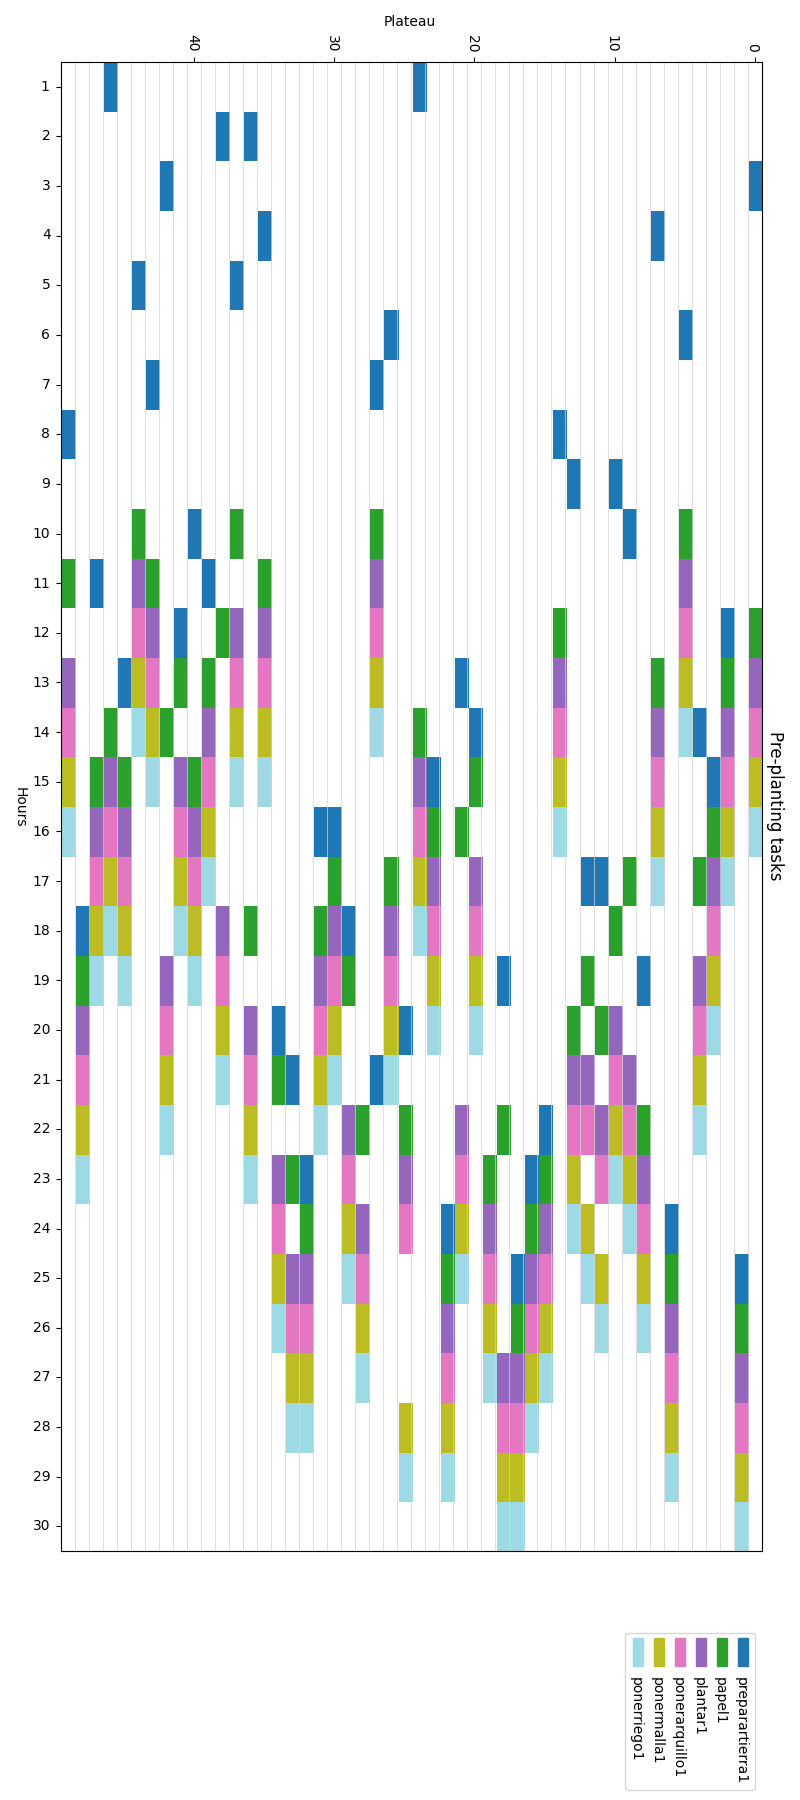
\includegraphics[scale=0.4]{img/grafico_pre_siembra1.png}
    \caption{Results obtained}
    \label{fig:resultados_pre1}
\end{figure}
\begin{figure}[ht!]
    \centering
    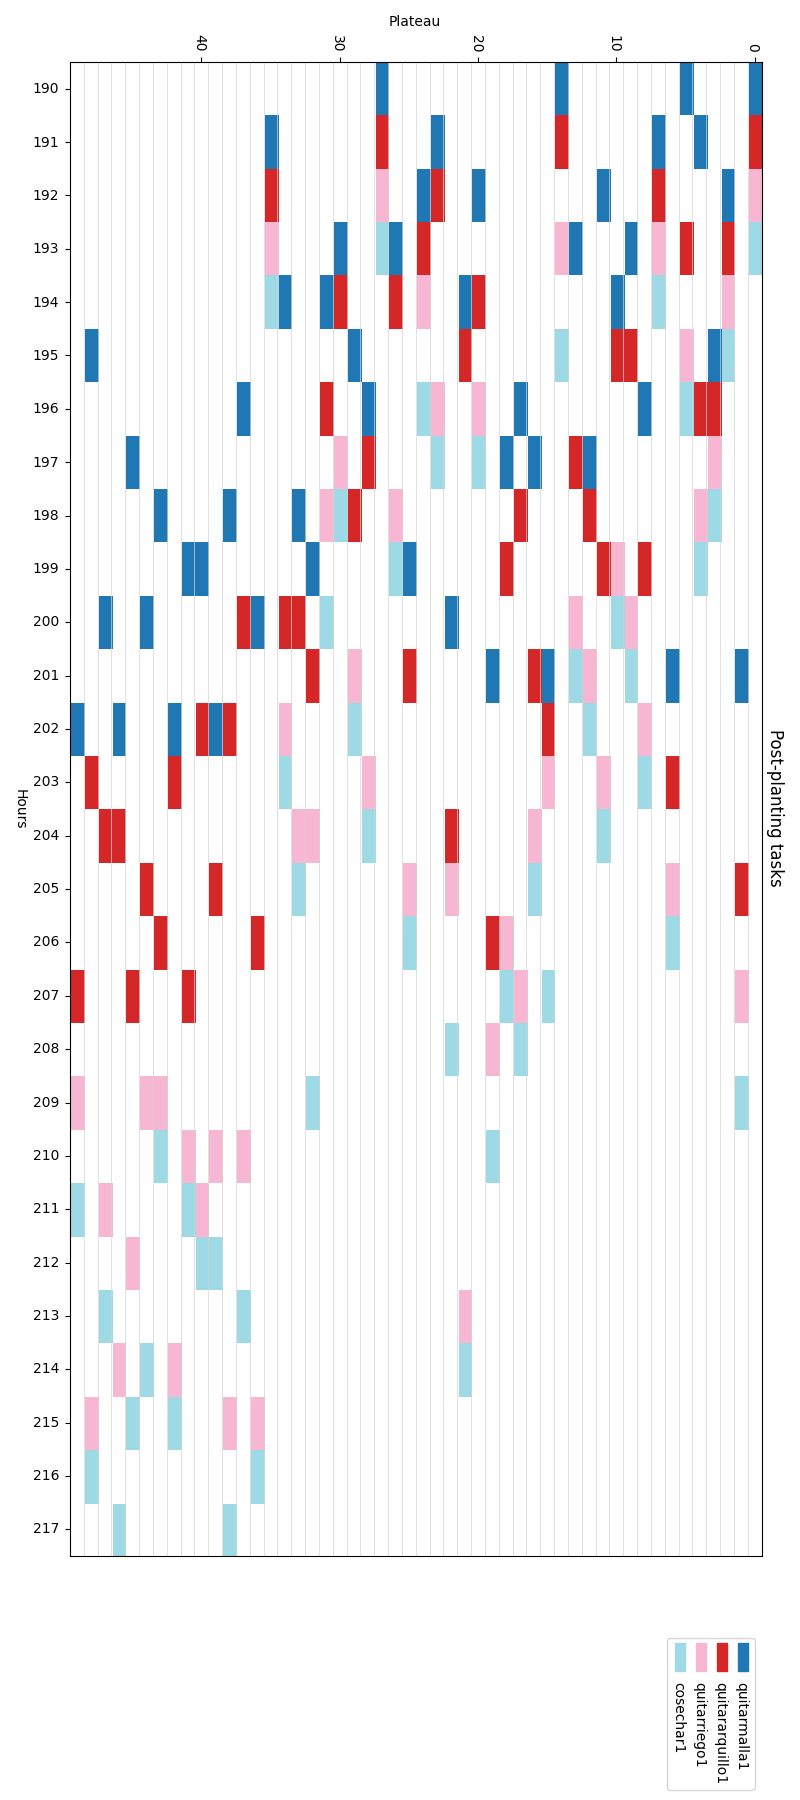
\includegraphics[scale=0.4]{img/grafico_post_siembra1.png}
    \caption{Results obtained}
    \label{fig:resultados_post1}
\end{figure}

\begin{figure}[ht!]
    \centering
    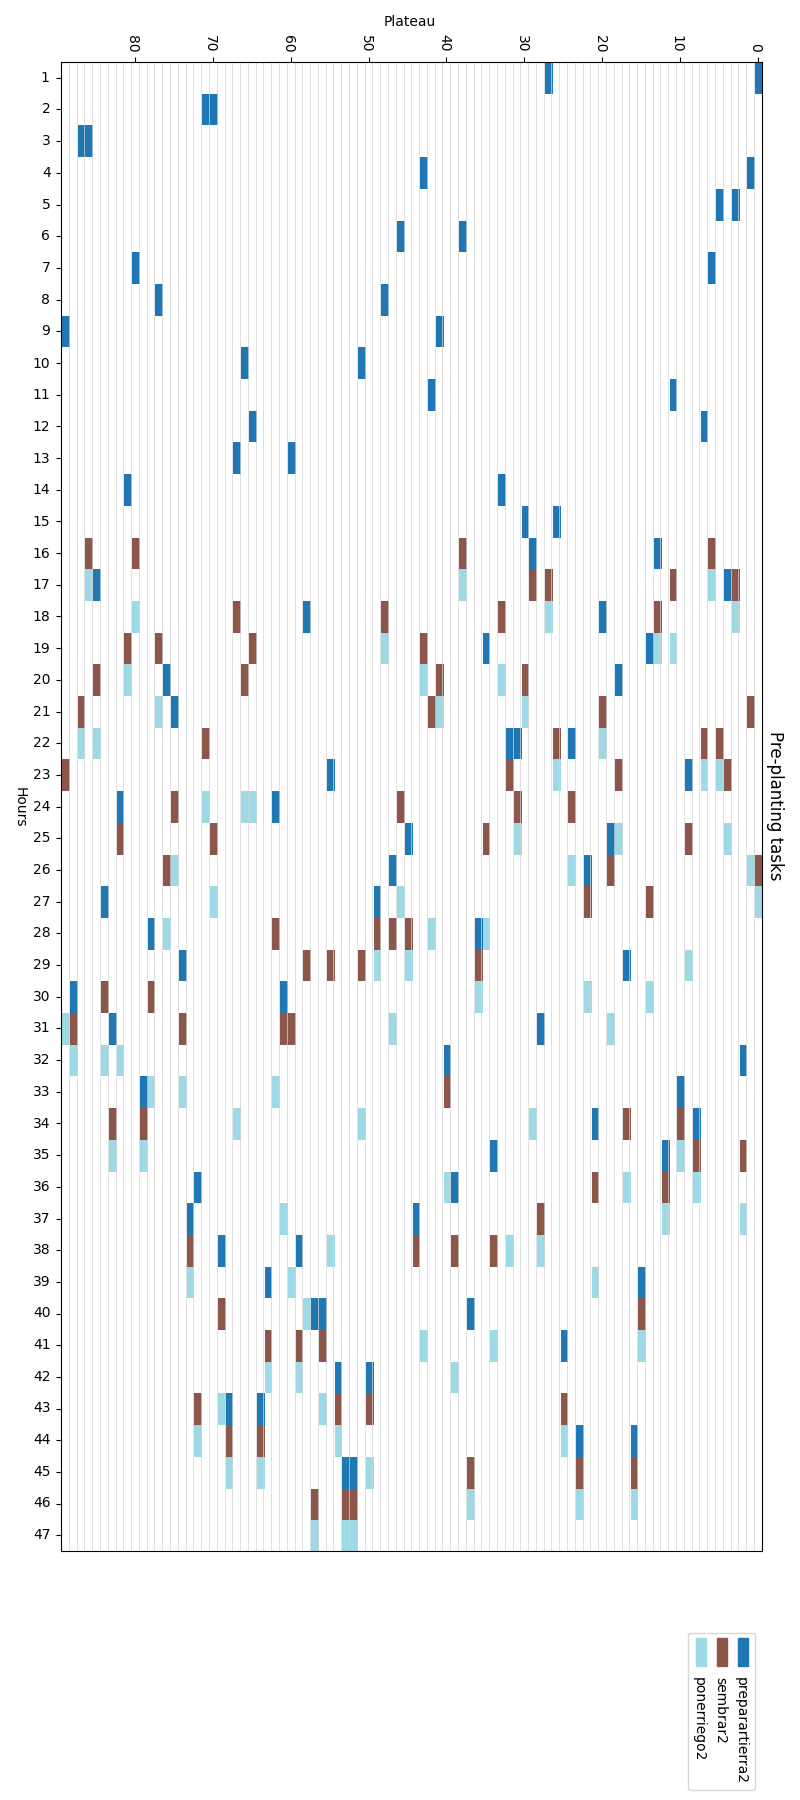
\includegraphics[scale=0.4]{img/grafico_pre_siembra2.png}
    \caption{Results obtained}
    \label{fig:resultados_pre2}
\end{figure}
\begin{figure}[ht!]
    \centering
    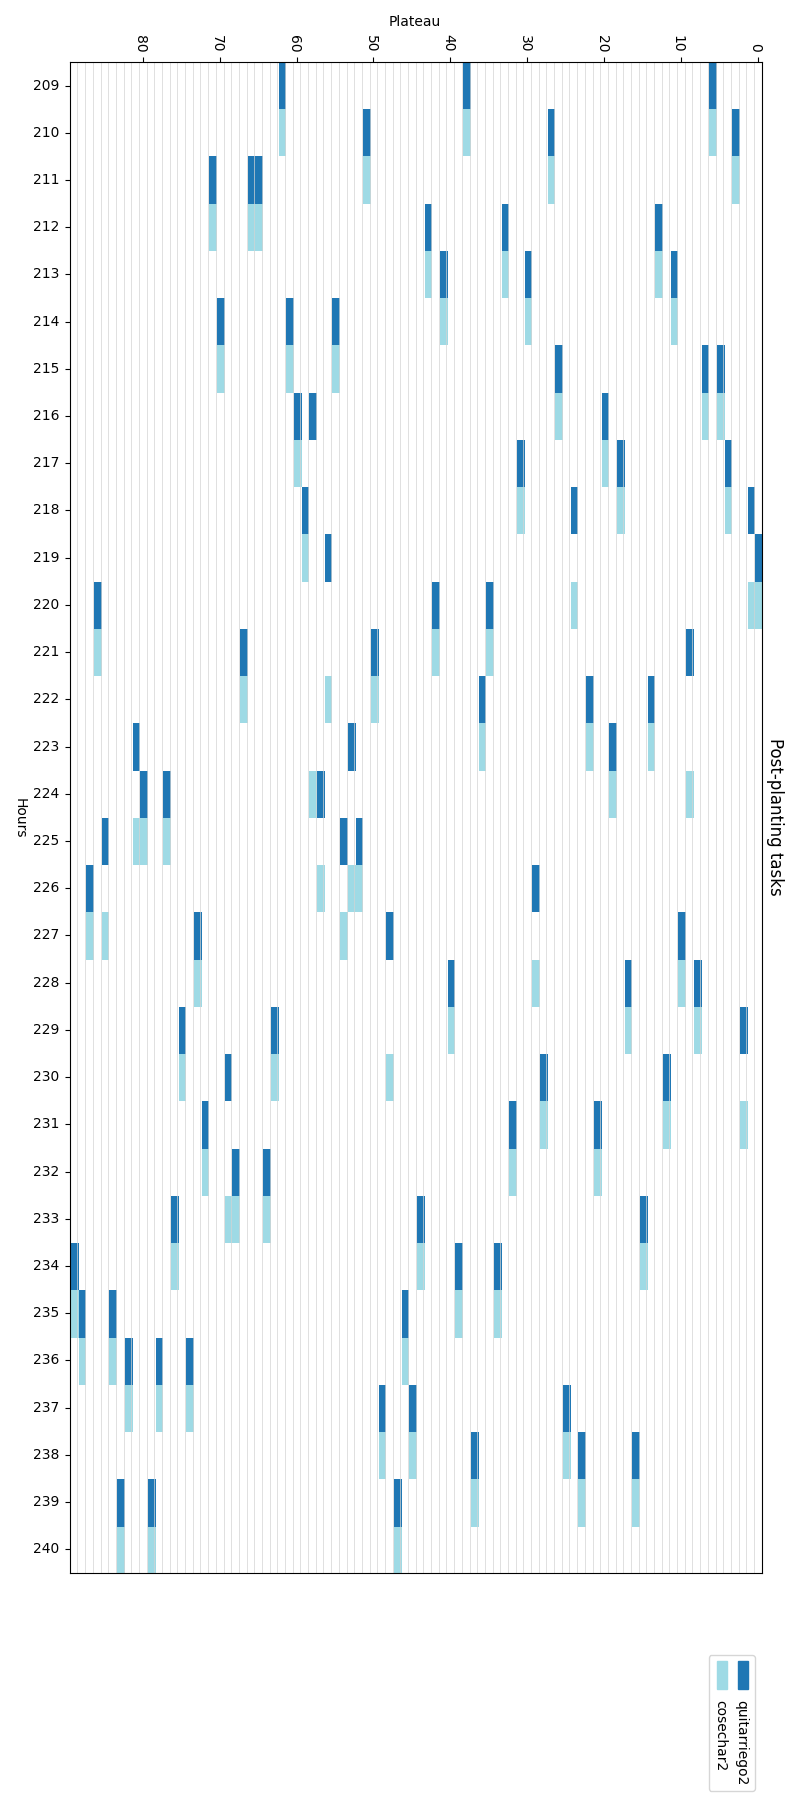
\includegraphics[scale=0.4]{img/grafico_post_siembra2.png}
    \caption{Results obtained}
    \label{fig:resultados_post2}
\end{figure}


\chapter*{Conclusion}
\addcontentsline{toc}{chapter}{7. Conclusion} % Manual index entry
This work has made it possible to address a real agricultural scheduling problem from a mathematical perspective,  
applying optimization tools to improve work organization at the company Intercrop.  
Through the analysis of the various tasks required for the cultivation of lettuce and spinach—two key products in the company's production—  
the operational complexity involved in coordinating teams, machinery, and execution times has been highlighted.

Throughout the project, a simplified but representative model has been developed,  
with the main objective of minimizing idle time between work groups.  
This approach addresses a problem observed directly in the field:  
the existence of unnecessary waiting periods when a task cannot begin until another one is completed.  
These idle hours, although inevitable to some extent, represent a direct cost to the company and reduce the overall efficiency of the production system.

The model has been built considering two independent fields, each with its own production line,  
and a task sequence that spans from soil preparation to harvesting.  
Despite the simplifications introduced—such as the standardization of field sizes,  
the absence of adverse weather conditions, or the strict separation between work groups—  
the approach retains a logical structure that remains faithful to the real process,  
allowing for practical and scalable conclusions to be drawn.

The development of this work has demonstrated how the mathematical knowledge acquired in the classroom can be successfully applied to real-world problems,  
providing concrete and quantifiable solutions to everyday situations in professional environments.  
Moreover, it has opened an interesting path for further exploration of the use of optimization models in agricultural contexts,  
where efficient decision-making can lead to significant improvements in performance and profitability.

In future phases, additional elements could be incorporated into the model, such as climate variability,  
mechanical failures, or the partial availability of machinery and personnel.  
It would also be interesting to extend the study to multiple interconnected fields or to explore more flexible strategies for staff hiring and rotation.  
All of these enhancements would contribute to building an even more robust decision-making tool for the daily management of companies like Intercrop.

